\documentclass[tikz,border=8pt]{standalone}
\usepackage[T1]{fontenc}
\usepackage{underscore}
\usetikzlibrary{arrows.meta,positioning,calc,fit}

\begin{document}
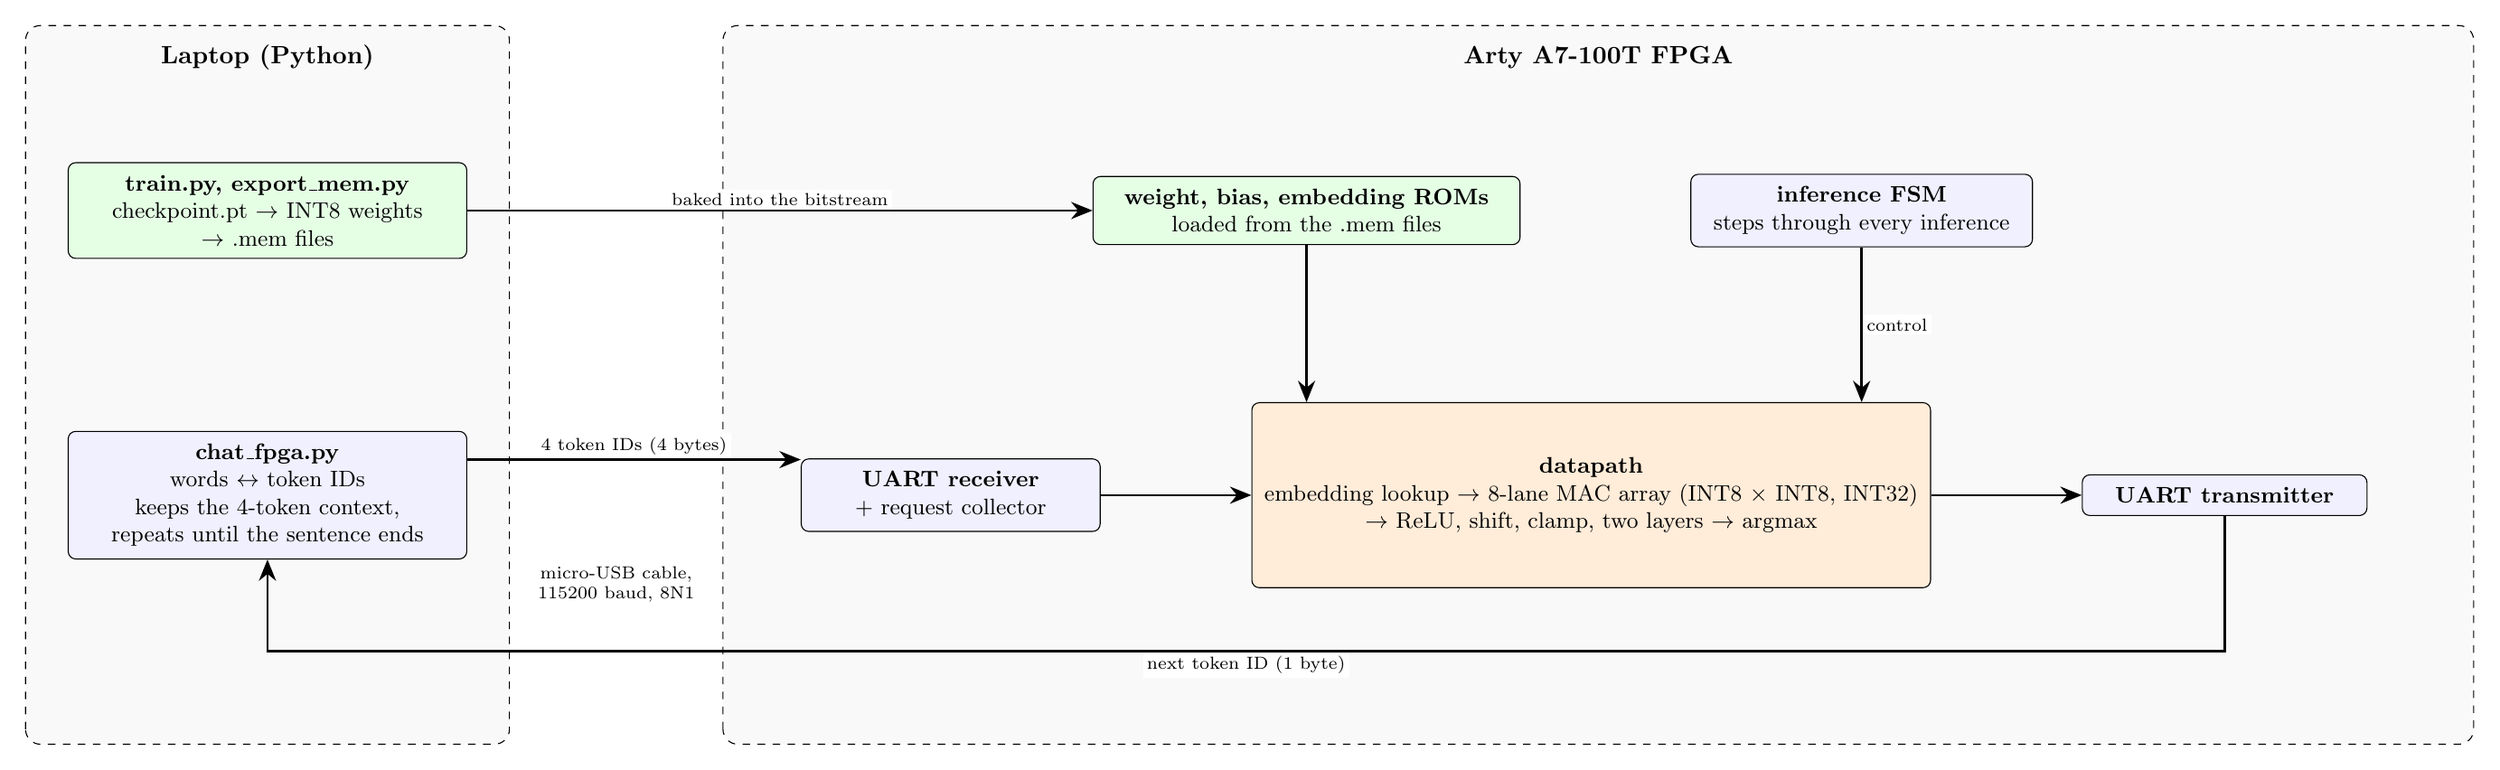
\begin{tikzpicture}[>={Stealth[length=3mm,width=2.4mm]},
  box/.style={draw,rounded corners=3pt,align=center,fill=blue!6,font=\small,inner sep=5pt},
  file/.style={box,fill=green!10},
  hw/.style={box,fill=orange!15},
  data/.style={->,line width=1pt},
  lab/.style={font=\scriptsize,fill=white,inner sep=1.5pt,align=center}]

\draw[dashed,rounded corners=6pt,fill=gray!5] (-3.4,-4.3) rectangle (3.4,5.8);
\node[font=\bfseries] at (0,5.35) {Laptop (Python)};
\draw[dashed,rounded corners=6pt,fill=gray!5] (6.4,-4.3) rectangle (31.0,5.8);
\node[font=\bfseries] at (18.7,5.35) {Arty A7-100T FPGA};

\node[file,minimum width=5.6cm] (train) at (0,3.2) {\textbf{train.py, export\_mem.py}\\checkpoint.pt $\to$ INT8 weights\\$\to$ .mem files};
\node[box,minimum width=5.6cm]  (chat)  at (0,-0.8) {\textbf{chat\_fpga.py}\\words $\leftrightarrow$ token IDs\\keeps the 4-token context,\\repeats until the sentence ends};

\node[box,minimum width=4.2cm]  (rx)    at (9.6,-0.8)  {\textbf{UART receiver}\\+ request collector};
\node[hw,minimum width=8.8cm,minimum height=2.6cm] (path) at (18.6,-0.8) {\textbf{datapath}\\embedding lookup $\to$ 8-lane MAC array (INT8 $\times$ INT8, INT32)\\$\to$ ReLU, shift, clamp, two layers $\to$ argmax};
\node[box,minimum width=4.0cm]  (tx)    at (27.5,-0.8) {\textbf{UART transmitter}};
\node[file,minimum width=6.0cm] (rom)   at (14.6,3.2)  {\textbf{weight, bias, embedding ROMs}\\loaded from the .mem files};
\node[box,minimum width=4.8cm]  (fsm)   at (22.4,3.2)  {\textbf{inference FSM}\\steps through every inference};

\draw[data] (train.east) -- node[above,lab]{baked into the bitstream} (rom.west);
\draw[data] (rom.south) -- (rom.south |- path.north);
\draw[data] (fsm.south) -- node[right,lab]{control} (fsm.south |- path.north);
\draw[data] (chat.east |- 0,-0.3) -- node[above,lab]{4 token IDs (4 bytes)} (rx.west |- 0,-0.3);
\draw[data] (rx) -- (path);
\draw[data] (path) -- (tx);
\draw[data] (tx.south) -- ++(0,-1.9) -| node[pos=0.25,below,lab]{next token ID (1 byte)} (chat.south);

\node[font=\scriptsize,fill=white,inner sep=2pt,align=center] at (4.9,-2.05) {micro-USB cable,\\115200 baud, 8N1};
\end{tikzpicture}
\end{document}
